% Chapter 4: Experimental Procedure 
\chapter{Apparatus and Experimental Procedure}
\label{chapter:experimental-procedure}

\graphicspath{ {report/C4 Experimental Procedure/assets/} } 

\section{BCI Apparatus}

In general, EEG-based BCI systems are comprised of the following core elements \cite{teplan-eeg-measurement}, \cite{bci-survey-nicolas-alonso}:
\begin{itemize}
    \item electrodes: placed on the scalp of the subject to record raw electrical potentials. 
    \item signal processing elements: amplifiers and filters are typically employed before the signals are digitised
    \item analogue-to-digital converter (ADC): digitises measured signal for manipulation in a computer or microcontroller
    \item computer or microcontroller: facilitates data processing, computation and storage
\end{itemize}

\subsection{OpenBCI Ganglion}
As the Imperial NGNI hardware prototype was still under development for a large part of this project, experimentation was initially done on a Ganglion bio-sensing kit made by \href{https://shop.openbci.com/products/ganglion-board?variant=13461804483}{OpenBCI} (OpenBCI, New York, USA). This kit was chosen due to the fact that it is relatively low-cost at 374.99 USD, open-source and has been scientifically validated as in \cite{autthasan-single-chan-ssvep}, \cite{peterson-bci-survey}. Furthermore, it is a relatively simple platform with sensing capabilities that are likely the most comparable to those anticipated for the NGNI prototype.

\begin{figure}
     \begin{subfigure}[c]{0.45\textwidth}
         \centering
         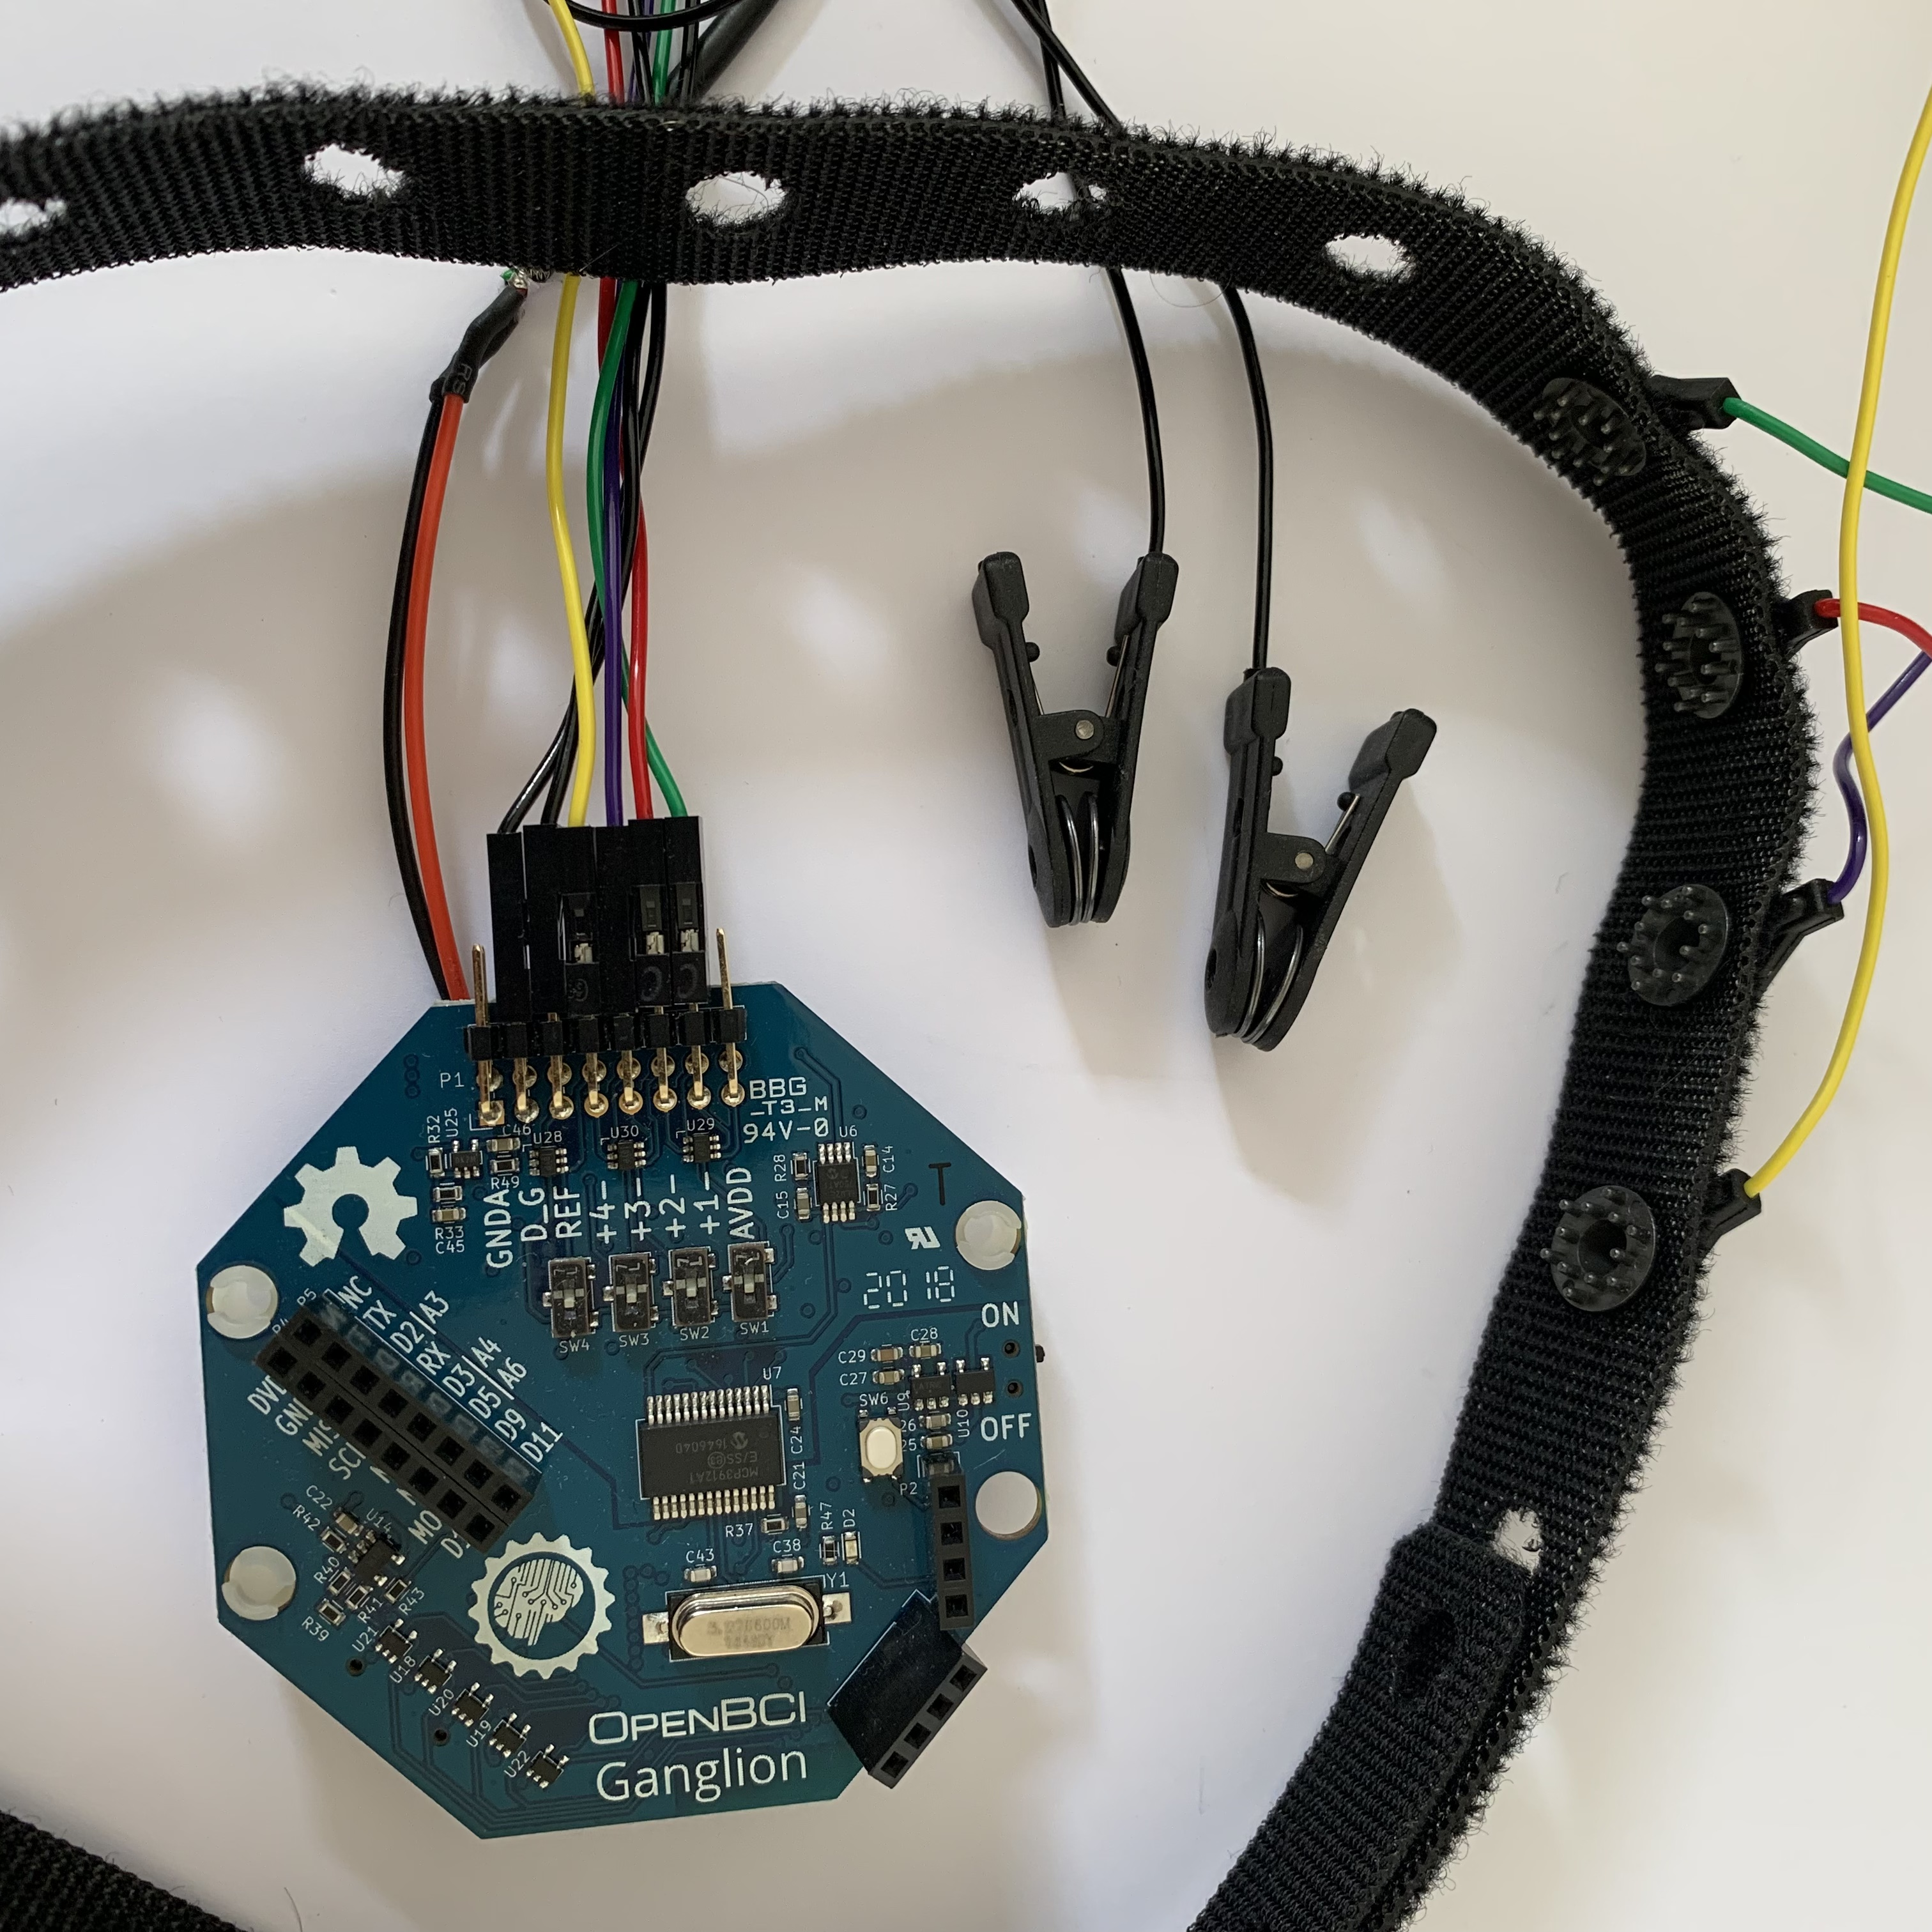
\includegraphics[width=\textwidth]{openbci}
         \caption{OpenBCI Ganglion board, electrodes and adjustable Velcro headband}
         \label{fig:openbci}
     \end{subfigure}
     \hfill
    \begin{subfigure}[c]{0.45\textwidth}
         \centering
         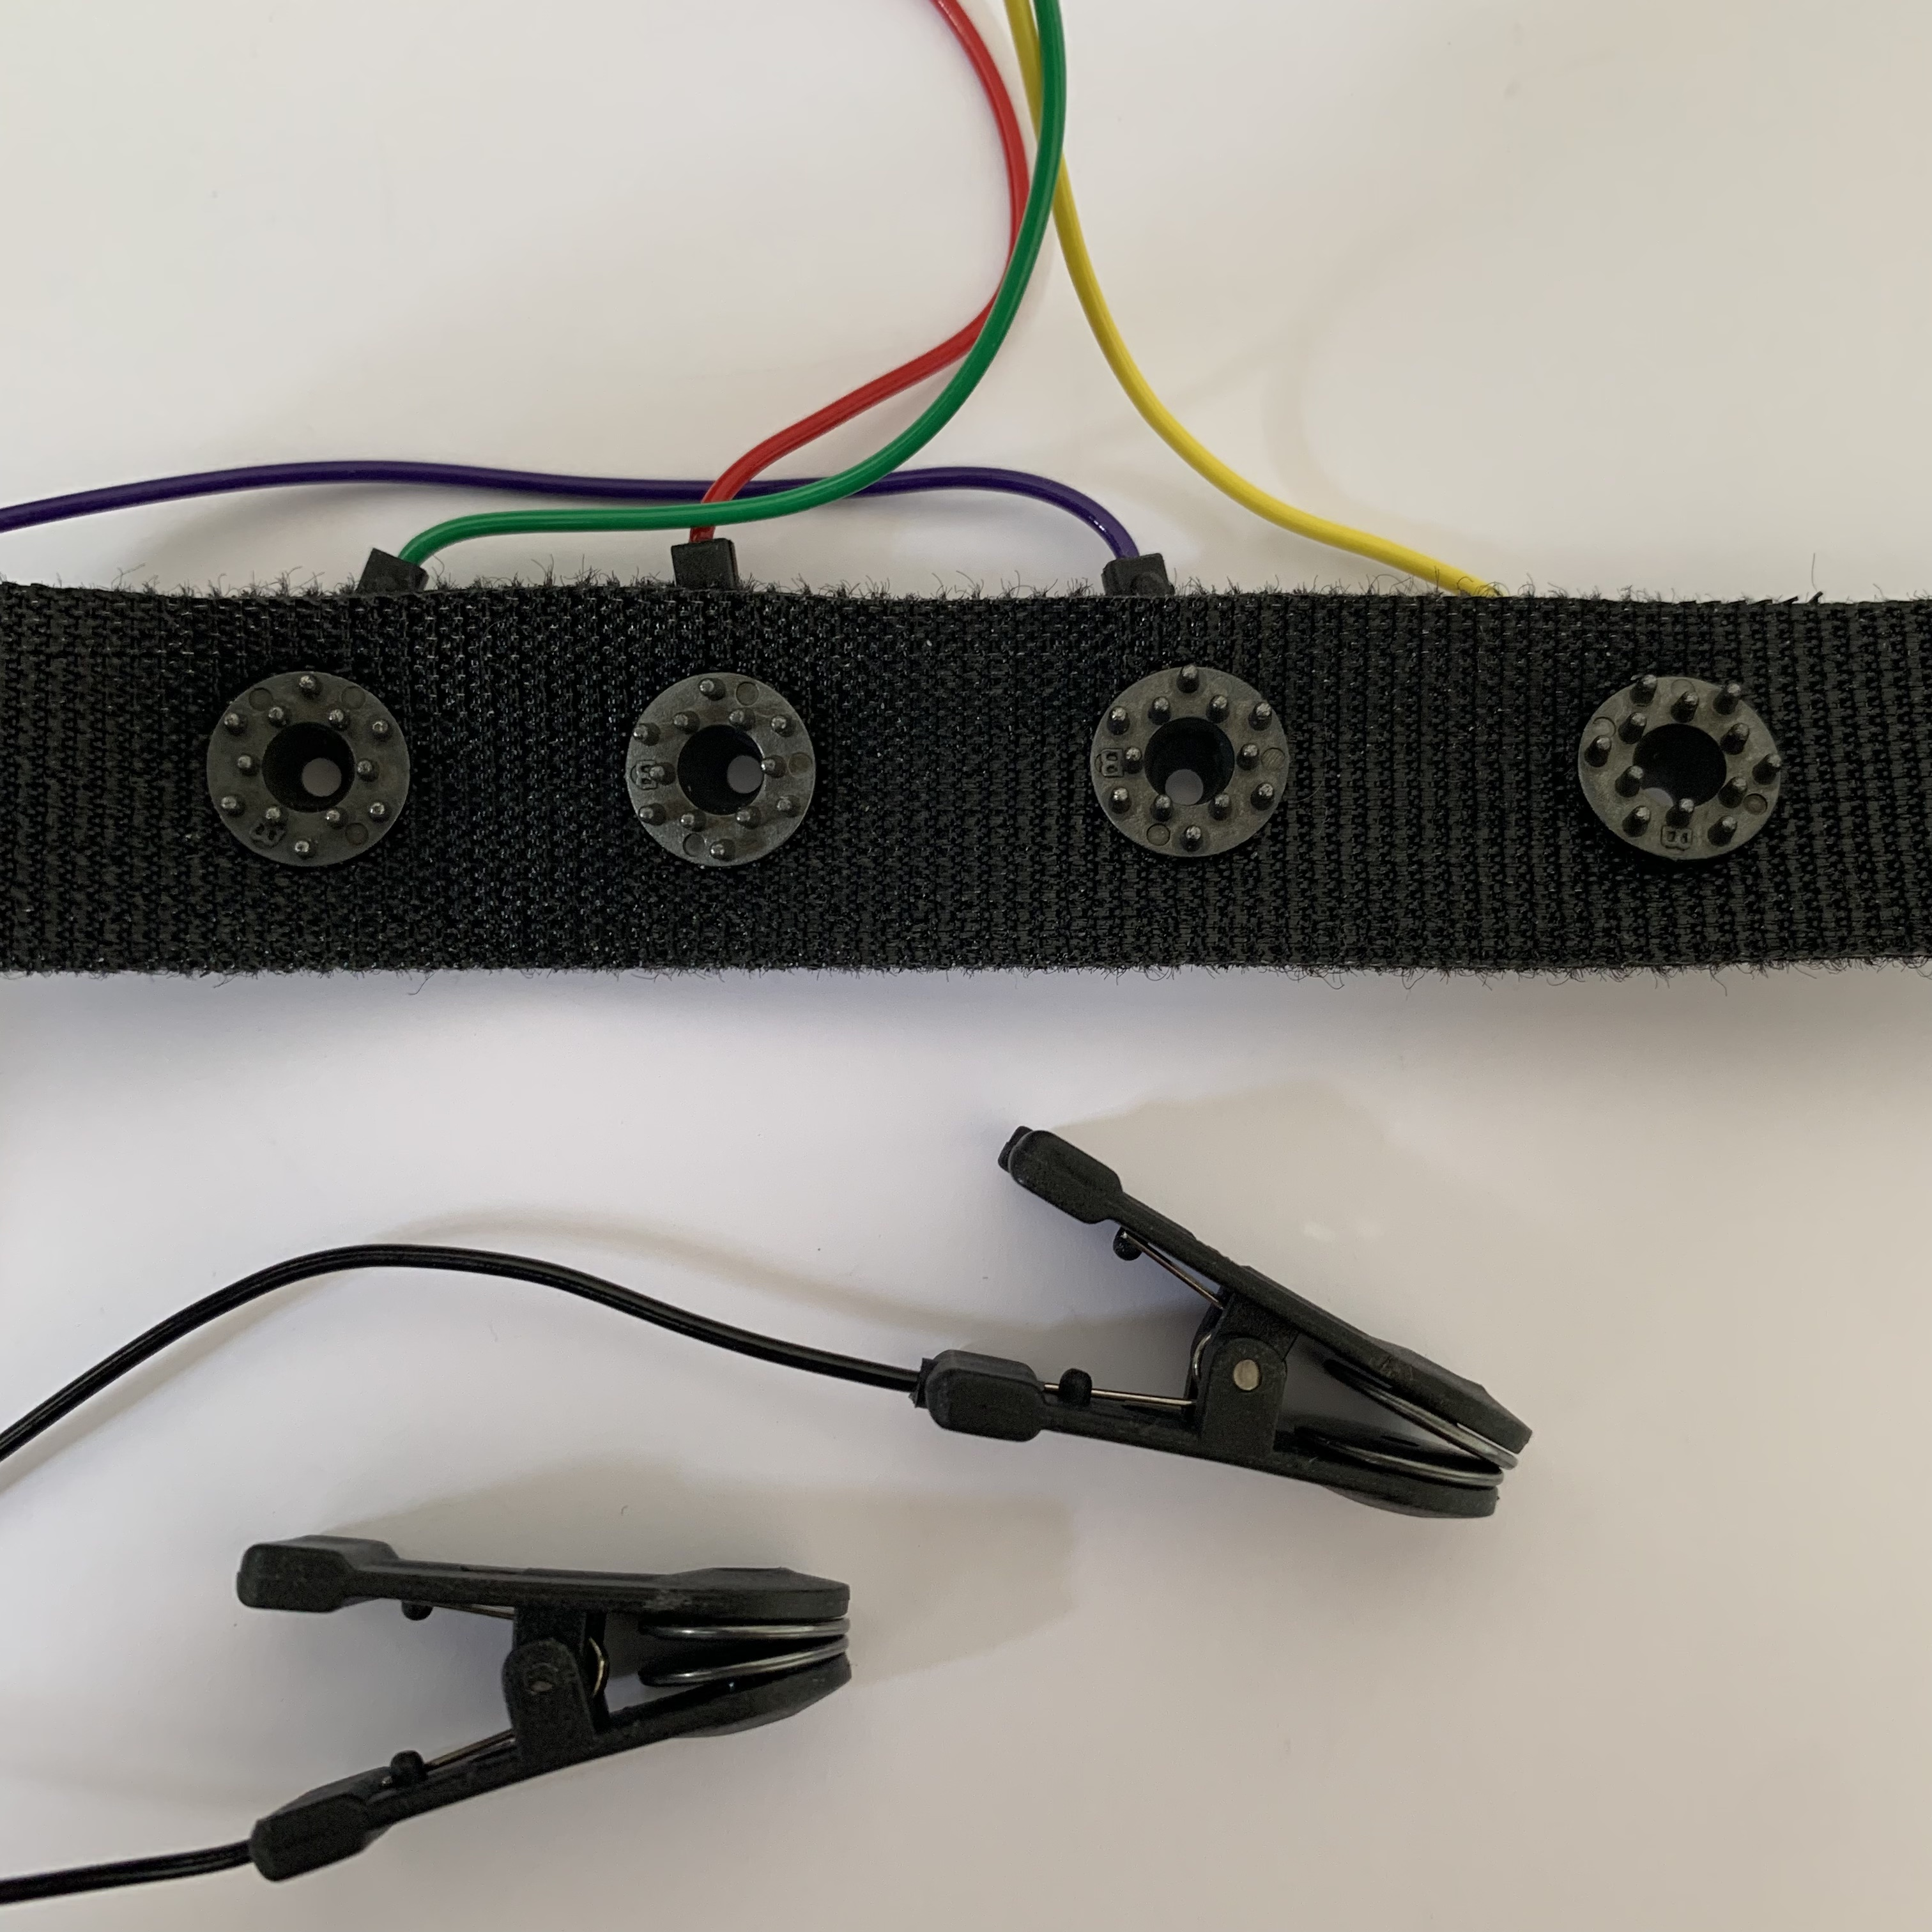
\includegraphics[width=\textwidth]{openbci-electrodes}
         \caption{Close-up view of the 4 active electrodes and two reference electrode clips (bottom)}
         \label{fig:openbci-electrodes}
     \end{subfigure}
        \caption[Images of the OpenBCI Ganglion bio-sensing device and electrodes]{Images of the OpenBCI Ganglion bio-sensing device and electrodes. The two black clips are the reference electrodes and the four active channels are received through the coloured wires.}
        \label{fig:openbci-subfigs}
\end{figure}
As depicted in Figure \ref{fig:openbci-subfigs}, the Ganglion board offers four active channels that. All four channels were using during experimentation as it was more convenient to exclude data from certain channels in post-processing than only measuring a subset of channels. Although wet electrodes can also be used with this kit, in accordance with the project constraints mentioned in Chapter \ref{chapter:introduction}, dry electrodes were used. As seen in Figure \ref{fig:openbci}, the four active electrodes have spiky nodules to increase surface pressure and thus improve contact quality with the scalp. For reference and comparison, some core features of the Ganglion board are provided below:
\begin{itemize}
    \item Microchip MCP3912 four channel 24-bit Delta-Sigma analogue frontend
    \item 200Hz sampling rate
    \item Simblee Bluetooth 4.0 module
\end{itemize}

\subsection{NGNI Prototype I}
\label{subsection:electronic-hardware-proto}
As alluded to in Chapter \ref{chapter:introduction}, the hardware to be used in this project was supplied by the Imperial NGNI Lab. All hardware prototypes developed by the Lab were based on the Espressif ESP32; a low-cost, low-power SoC (system-on-chip) based on the Tensilica Xtensa LX6 microprocessor with integrated Wi-Fi and Bluetooth. Features of the ESP32 that are relevant to this project include \cite{esp32-digikey}:
\begin{itemize}
    \item dual-core, 240MHz CPU
    \item onboard FPU
    \item 12-bit SAR ADC
    \item 4x SPI, 2x I2C, 3x UART interfaces
    \item up to 600 DMIPS performance
    \item ultra low-power (ULP) co-processor
    \item 4 MiB SRAM
    \item integrated Wi-Fi 802.11 b/g/n and BLE
\end{itemize}
The ESP32 is extremely capable for its low price tag of around 3.6 USD \cite{esp32-digikey}. Its dual-core CPU is also particularly attractive as it could allow decoding-related computation and network communication to happen concurrently.

Figure \ref{fig:esp-hardware} shows the electronic hardware prototype developed by the NGNI Lab. In this design, the active components directly involved in the normal functioning of the system are independently located on a `target' board. A second programmer board was created to enable serial communication with the target; most commonly in order to flash new firmware to it during development. The programmer board uses six spring-loaded pogo pins to make momentary contact with corresponding pads on the target board during development. These 6 pins, and their corresponding pads on the target board, can be seen directly in the centre of Figure \ref{fig:esp-hardware-both}. A 3D printed housing was created to facilitate correct contact between the boards during development. As depicted in the image of the programmer board in Figure \ref{fig:esp-hardware-programmer}, it also features contact points for probing a few selected pins/junctions on the target board such as: the ADC output, the inverting pin of the analogue amplifier, the output of the analogue filter and all relevant supply voltage references. In addition, two momentary push-buttons connected to the \texttt{BOOT0} and \texttt{EN} pins of the ESP32 SoC are included in order to allow hardware resets and to control the entry state upon reset: bootloader mode or normal operating mode. 

\begin{figure}[!htb]
     \centering
     \begin{subfigure}[b]{0.3\textwidth}
         \centering
         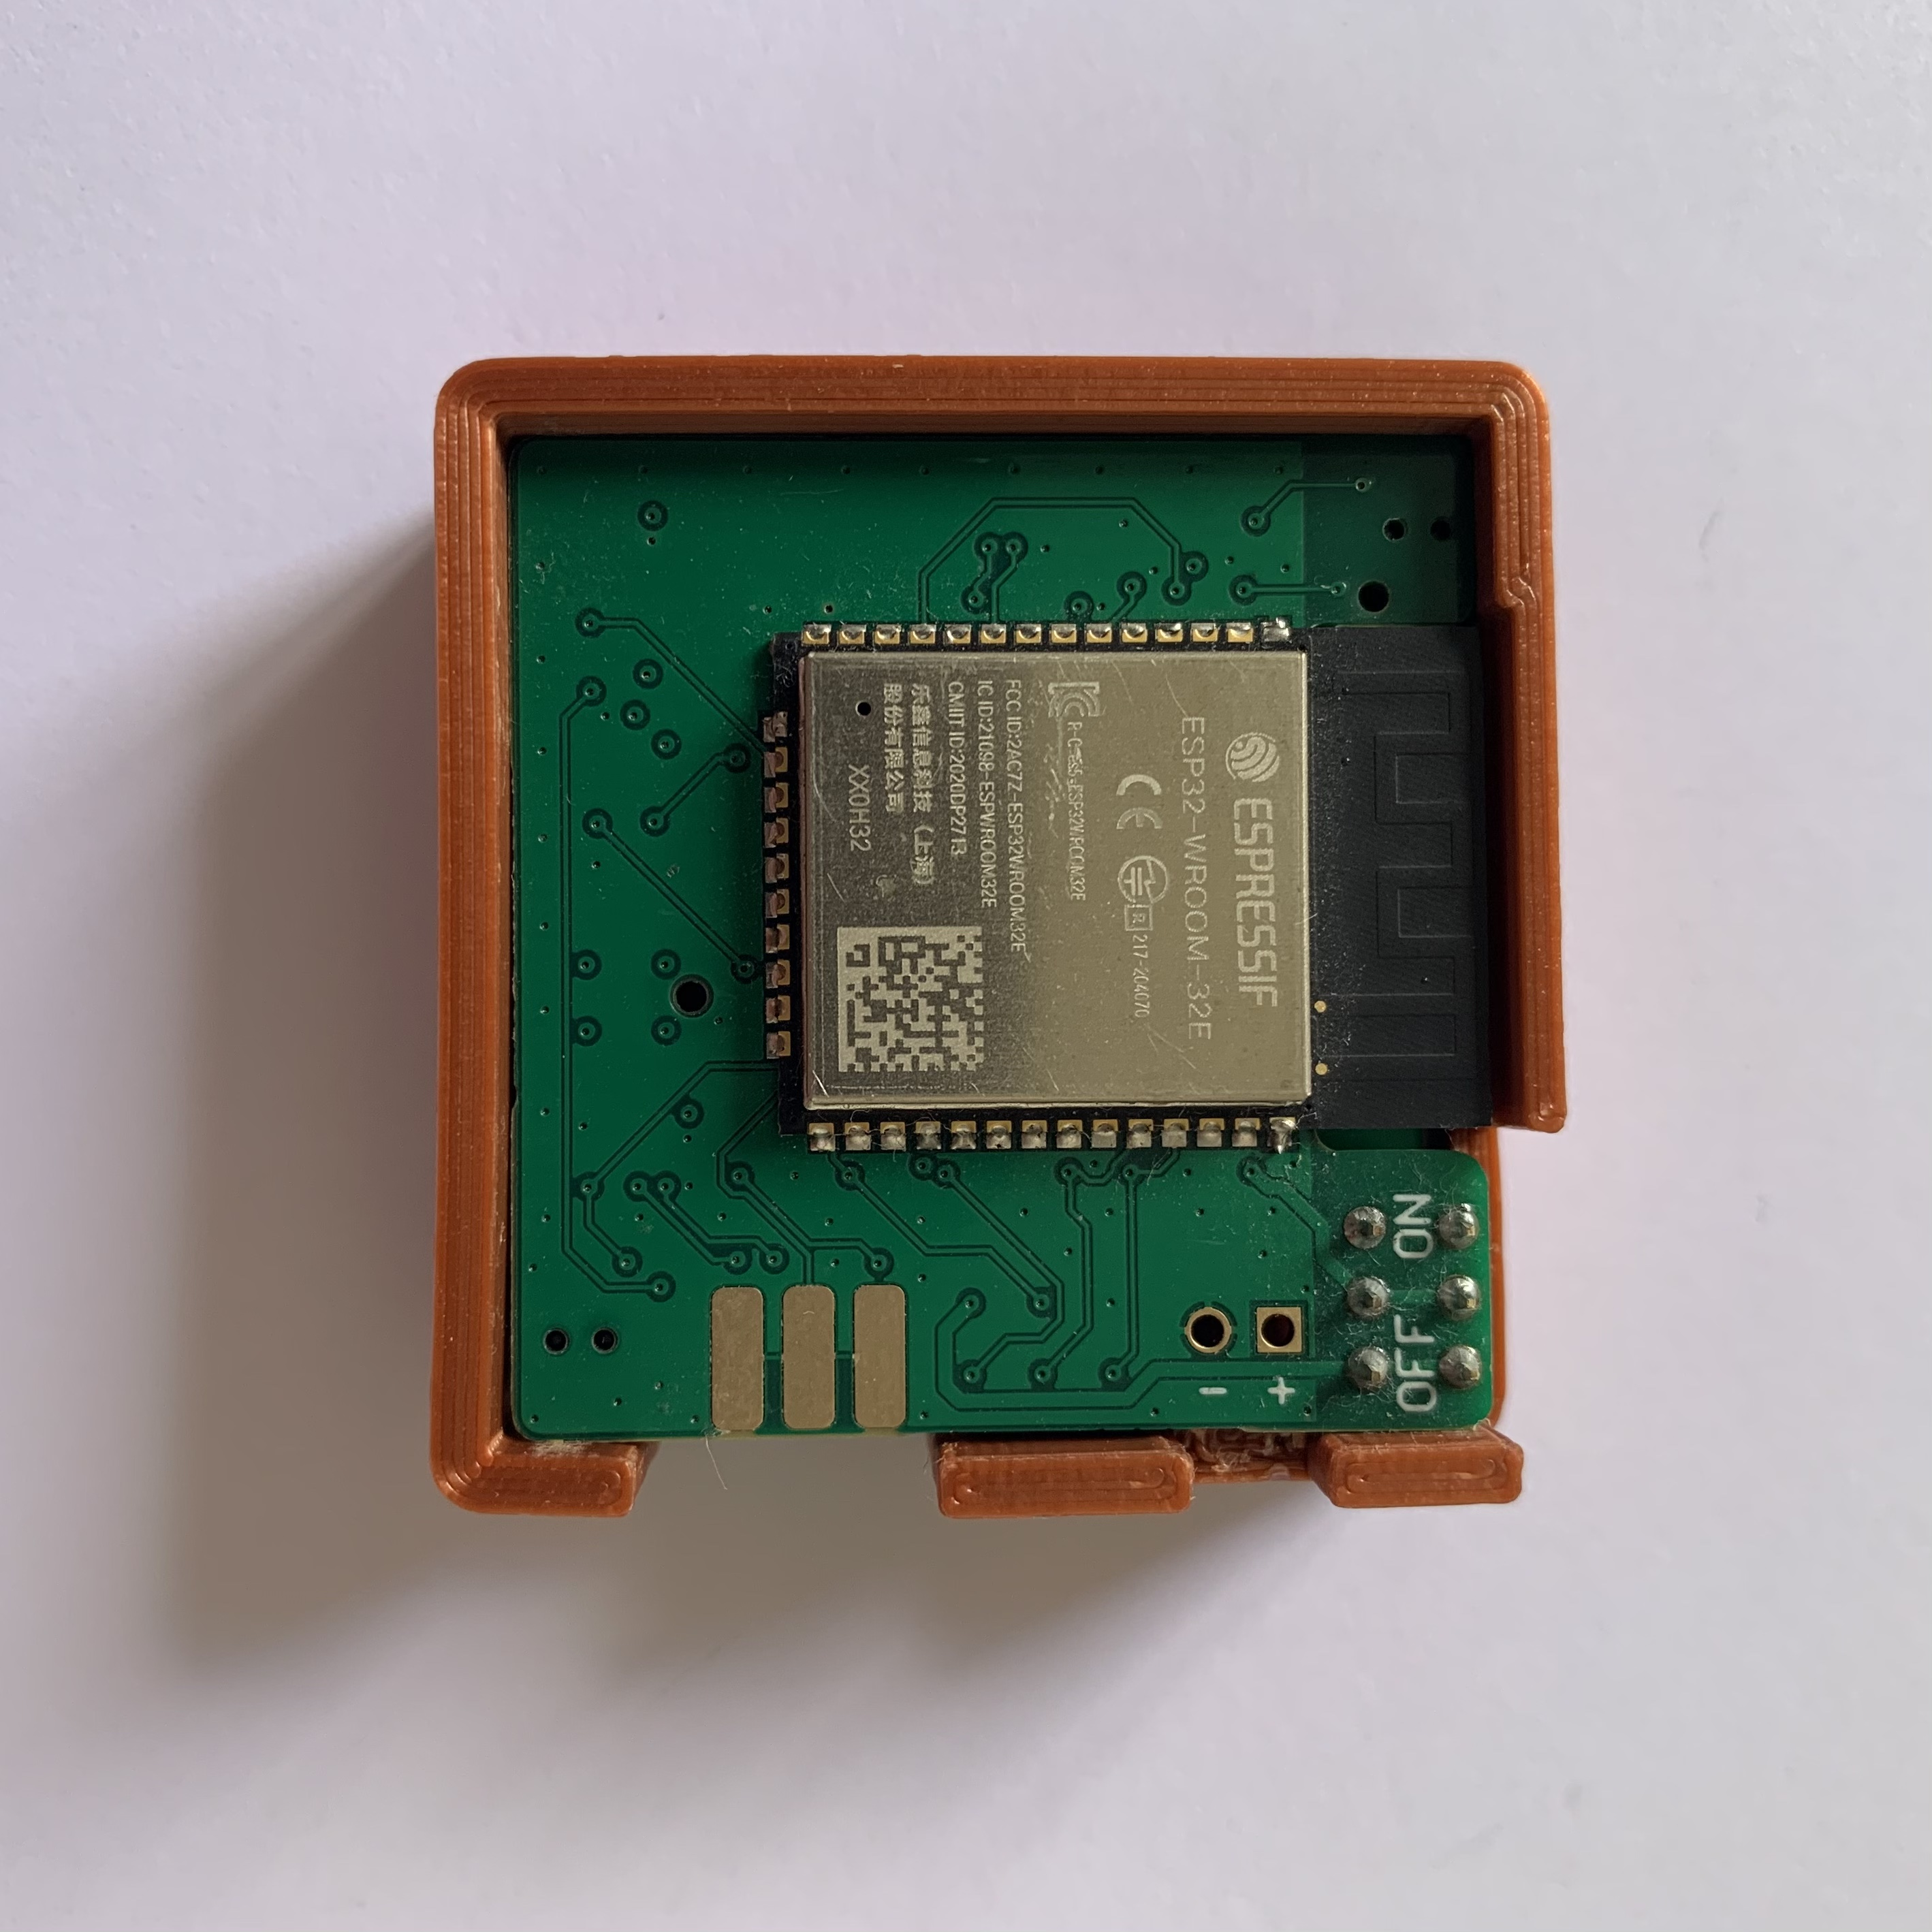
\includegraphics[width=\textwidth]{esp-top}
         \caption{Target board with ESP32 SoC and peripheral electronics}
         \label{fig:esp-hardware-soc}
     \end{subfigure}
     \hfill
     \begin{subfigure}[b]{0.3\textwidth}
         \centering
         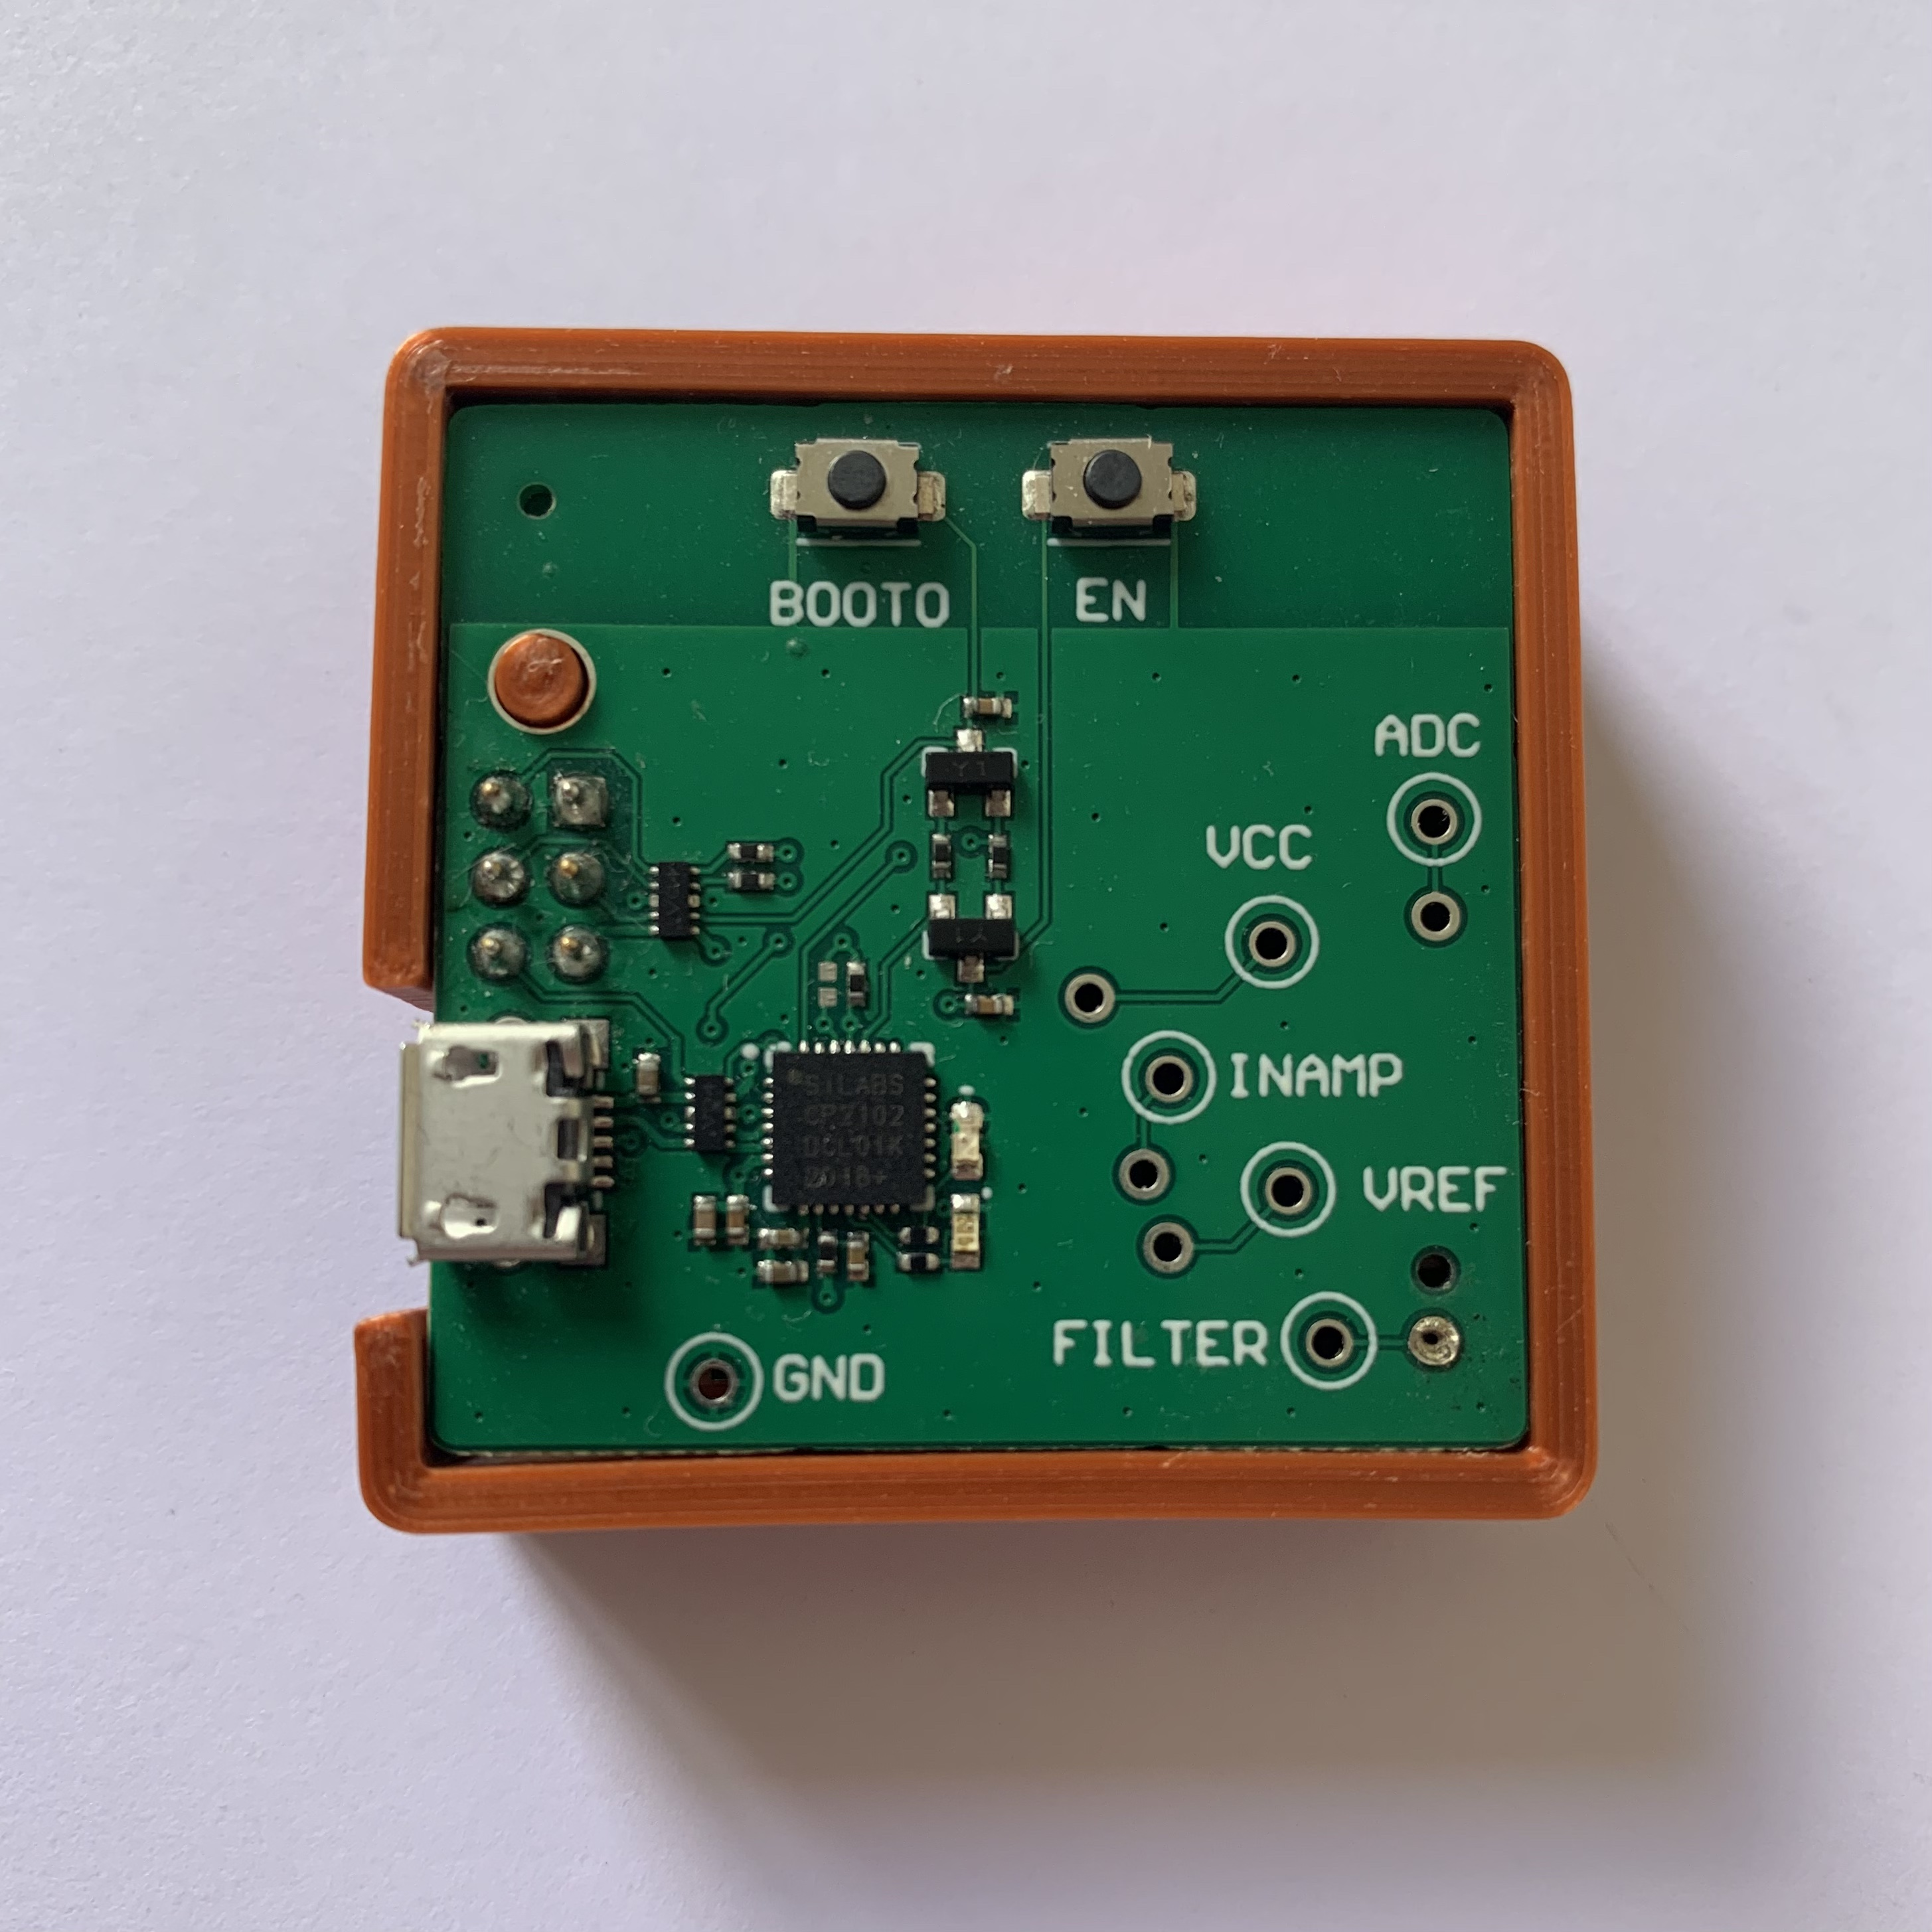
\includegraphics[width=\textwidth]{programmer}
         \caption{Programmer board with serial-to-USB interface }
         \label{fig:esp-hardware-programmer}
     \end{subfigure}
     \hfill
    \begin{subfigure}[b]{0.3\textwidth}
         \centering
         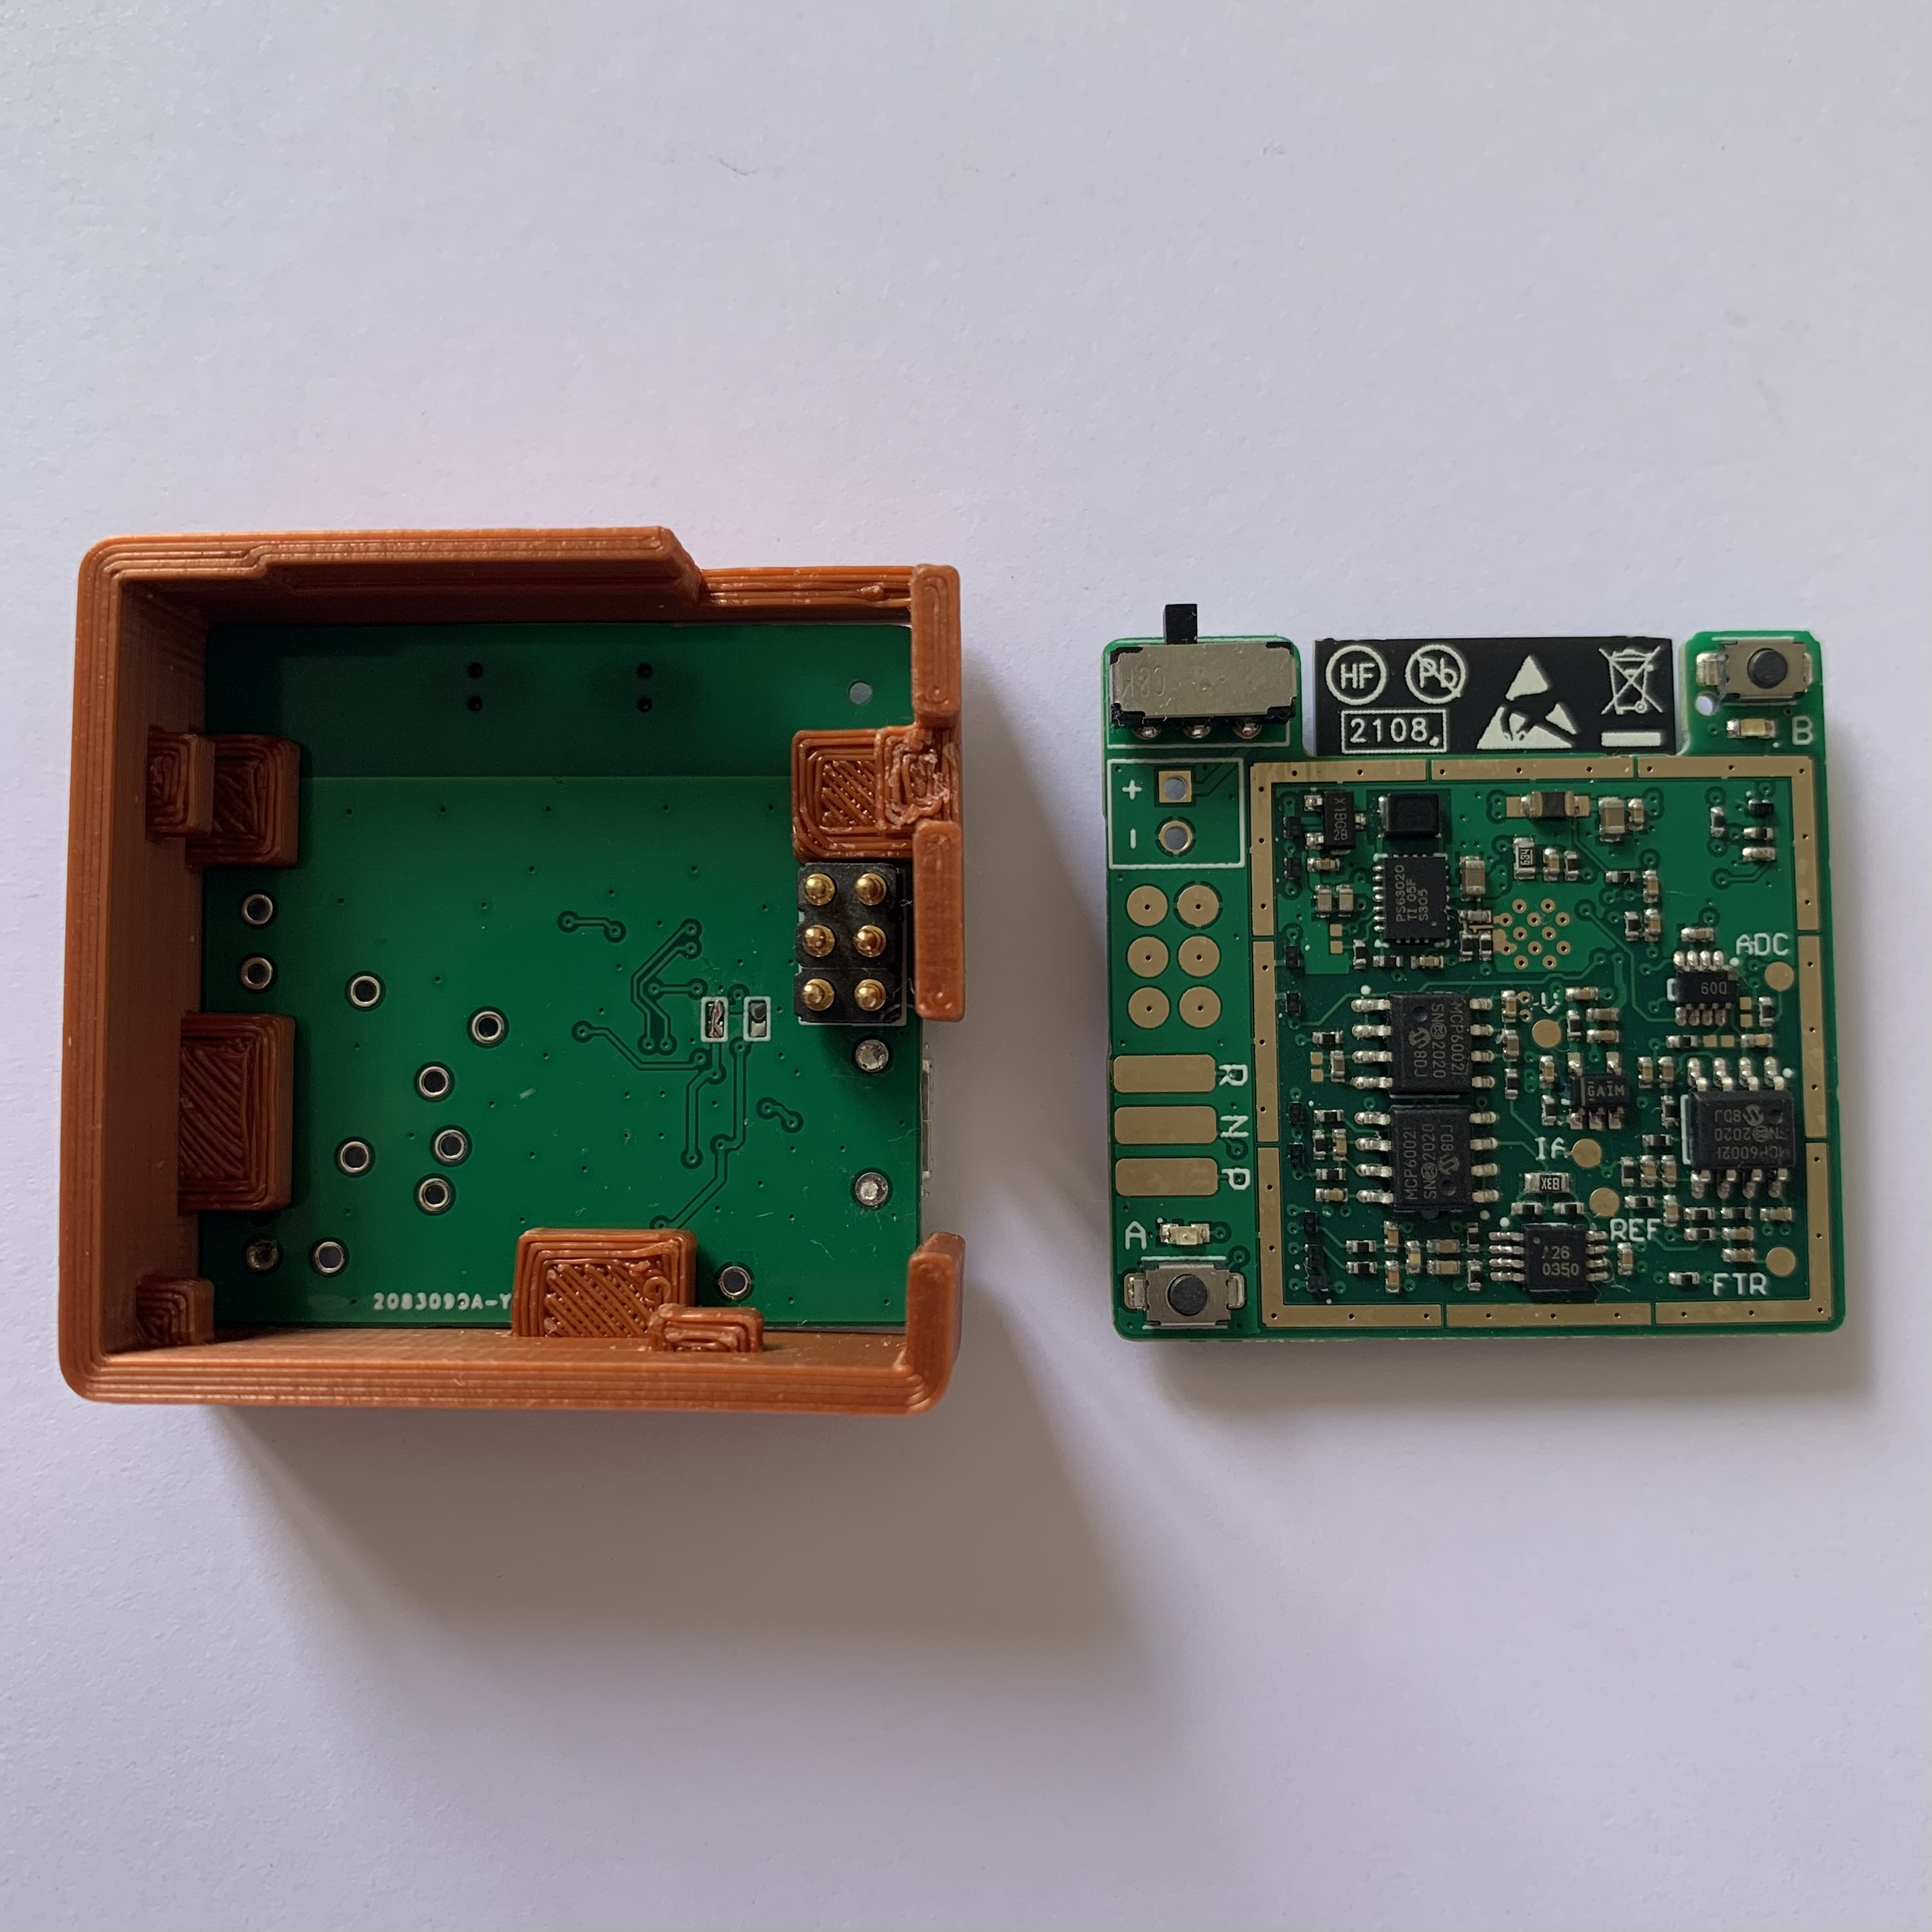
\includegraphics[width=\textwidth]{esp-both}
         \caption{Bottom side of the programmer board (left) and target board}
         \label{fig:esp-hardware-both}
     \end{subfigure}
        \caption[Images of the electronic hardware prototype developed in the Imperial NGNI Lab]{Images of the electronic hardware prototype developed in the Imperial NGNI Lab. This prototype includes the target board with ESP32 SoC, as well as a programmer board that is used to flash new firmware on to the microcontroller aboard the target board. The orange 3D-printed housing is used to position the programmer board above the target during firmware updates or other serial communication with an external computer.}
        \label{fig:esp-hardware}
\end{figure}

\subsubsection{Analogue signal processing system}

Figure \ref{fig:analogue-system-c4} provides an overview of the key analogue signal processing elements in the electronic hardware prototype. This system is primarily responsible for amplifying $\mu$V-scale raw EEG signals, filtering out 50Hz mains power interference and offering further amplification that can be adjusted in firmware. 

\begin{figure}
    \centering
    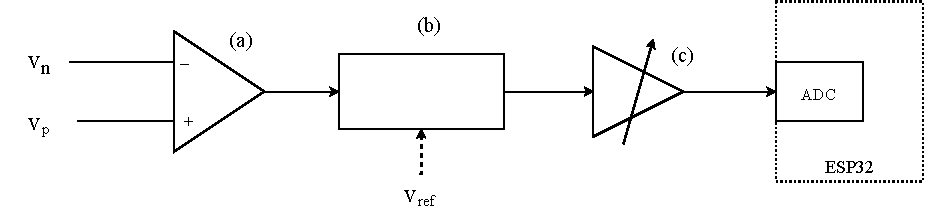
\includegraphics[width=\textwidth]{analogue-system}
    \caption[Functional overview diagram of the analogue signal processing system in the NGNI electronic hardware prototype.]{Functional overview diagram of the analogue signal processing system in the NGNI electronic hardware prototype. (a) signals captured from the two active electrodes, $\textrm{v}_n$ and $\textrm{v}_p$, first pass through a differential amplifier. (b) a third order hour glass low-pass filter is used for 50Hz mains power rejection. (c) the filtered signal can be further amplified with adjustable gain that is controlled via a digital potentiometer through a SPI interface.}
    \label{fig:analogue-system-c4}
\end{figure}

Important details of the components shown in Figure \ref{fig:analogue-system-c4} are provided below:

\begin{enumerate}[label=(\alph*)] % (a), (b), (c), ...
\item differential amplifier
\begin{itemize}
    \item fixed gain of 1120
    \item high-pass filter dynamics: highest corner frequency $f_c=0.48$Hz
\end{itemize}
\item hourglass low-pass filter
\begin{itemize}
    \item Q factor 2.17
    \item low-pass corner frequency $f_c=37.4$Hz
    \item notch frequency $f_n=50$Hz
    \item 50Hz rejection characteristics: minimum 17dB, nominal 35dB and maximum 55dB.
\end{itemize}

\item adjustable-gain output amplifier
\begin{itemize}
    \item adjustable gain between 1.745 and 19.2
    \item input low-pass filter dynamics: corner frequency of $f_c=36.35$Hz 
\end{itemize}
\end{enumerate}
Important to note is that the analogue hourglass filter designed for 50Hz rejection has a corner frequency of $f_c=37.4$Hz. Therefore, EEG signals with harmonics beyond $37.4$Hz will start to become attenuated as a side-effect of the dynamics of this filter. Furthermore, as mentioned in Section \ref{subsection:nature-of-eeg-signals}, raw EEG signals are expected to be in the range of 0.5 to 100$\mu$V peak-to-peak. Neglecting other minor sources of gain or attenuation in the system, the ranges of signal amplitudes (peak-to-peak voltages) at the output of the system for various input EEG signal amplitudes and gain configurations is shown in Table \ref{tab:gain-voltage-ranges}. Note that, with the minimum gain configuration of $g_2=1.745$ on the output amplifier, the maximum expected output voltage is only $v_{\textrm{out}}=0.132$V which is approximately equal to the full range of amplitudes expected with this configuration.

\begin{table}[]
\centering
\begin{tabular}{@{}lllll@{}}
\toprule
\textbf{$\mathbf{v_{\textrm{in}}}$} ($\mu$V) & \textbf{$\mathbf{g_1}$} & \textbf{$\mathbf{g_2}$} & \textbf{$\mathbf{g_1g_2}$} & \textbf{$\mathbf{v_{\textrm{out}}}$} ($\textrm{V}$)\\ \midrule
0.5          & 1120        & 1.745       & 1315.4          & \textbf{0.000658}        \\
0.5          & 1120        & 19.2        & 21504           & 0.0108          \\
100          & 1120        & 1.745       & 1315.4          & 0.132           \\
100          & 1120        & 19.2        & 21504           & \textbf{2.15}            \\ \bottomrule
\end{tabular}
\caption[Table showing the theoretical range of voltages measured at the ADC of the ESP32 for varying input signal magnitudes and gain configurations]{Table showing the theoretical range of voltages $v_{\textrm{out}}$ at the input to the ADC of the ESP32 (output of the analogue signal processing system) with varying input signal amplitude $v_{\textrm{in}}$ and gain configurations. Fixed gain $g_1$ is that of the input stage differential amplifier and $g_2$ is the adjustable gain of the output amplifier. The expected EEG signal amplitude range, $v_{\textrm{in}}$, is from \cite{teplan-eeg-measurement}. Voltages shown are peak-to-peak amplitudes.}
\label{tab:gain-voltage-ranges}
\end{table}

It should be noted that this first revision of the electronic hardware prototype is designed for coupling with \textit{two} active electrodes but only allows for \textit{differential} signal measurements between these electrodes. Consequently, only a single `channel' is recorded by the ADC in the ESP32. A third reference electrode is also expected in order to offer a common voltage reference point between the two active channels. 

\subsubsection{Mechanical hardware prototype}

The very first complete EEG headband prototype comprising electronic and mechanical hardware is shown in Figure \ref{fig:frankenstein-hardware}. This version did not include any means of adjusting the circumference of the band of the electrode positions within it besides having to drill new holes in it. As such, this makeshift prototype was more intended to serve as a preliminary means of gathering real-life data using the electronic hardware. It was not designed (nor expected) to produce viable results for SSVEP decoding. 

\begin{figure}
    \centering
    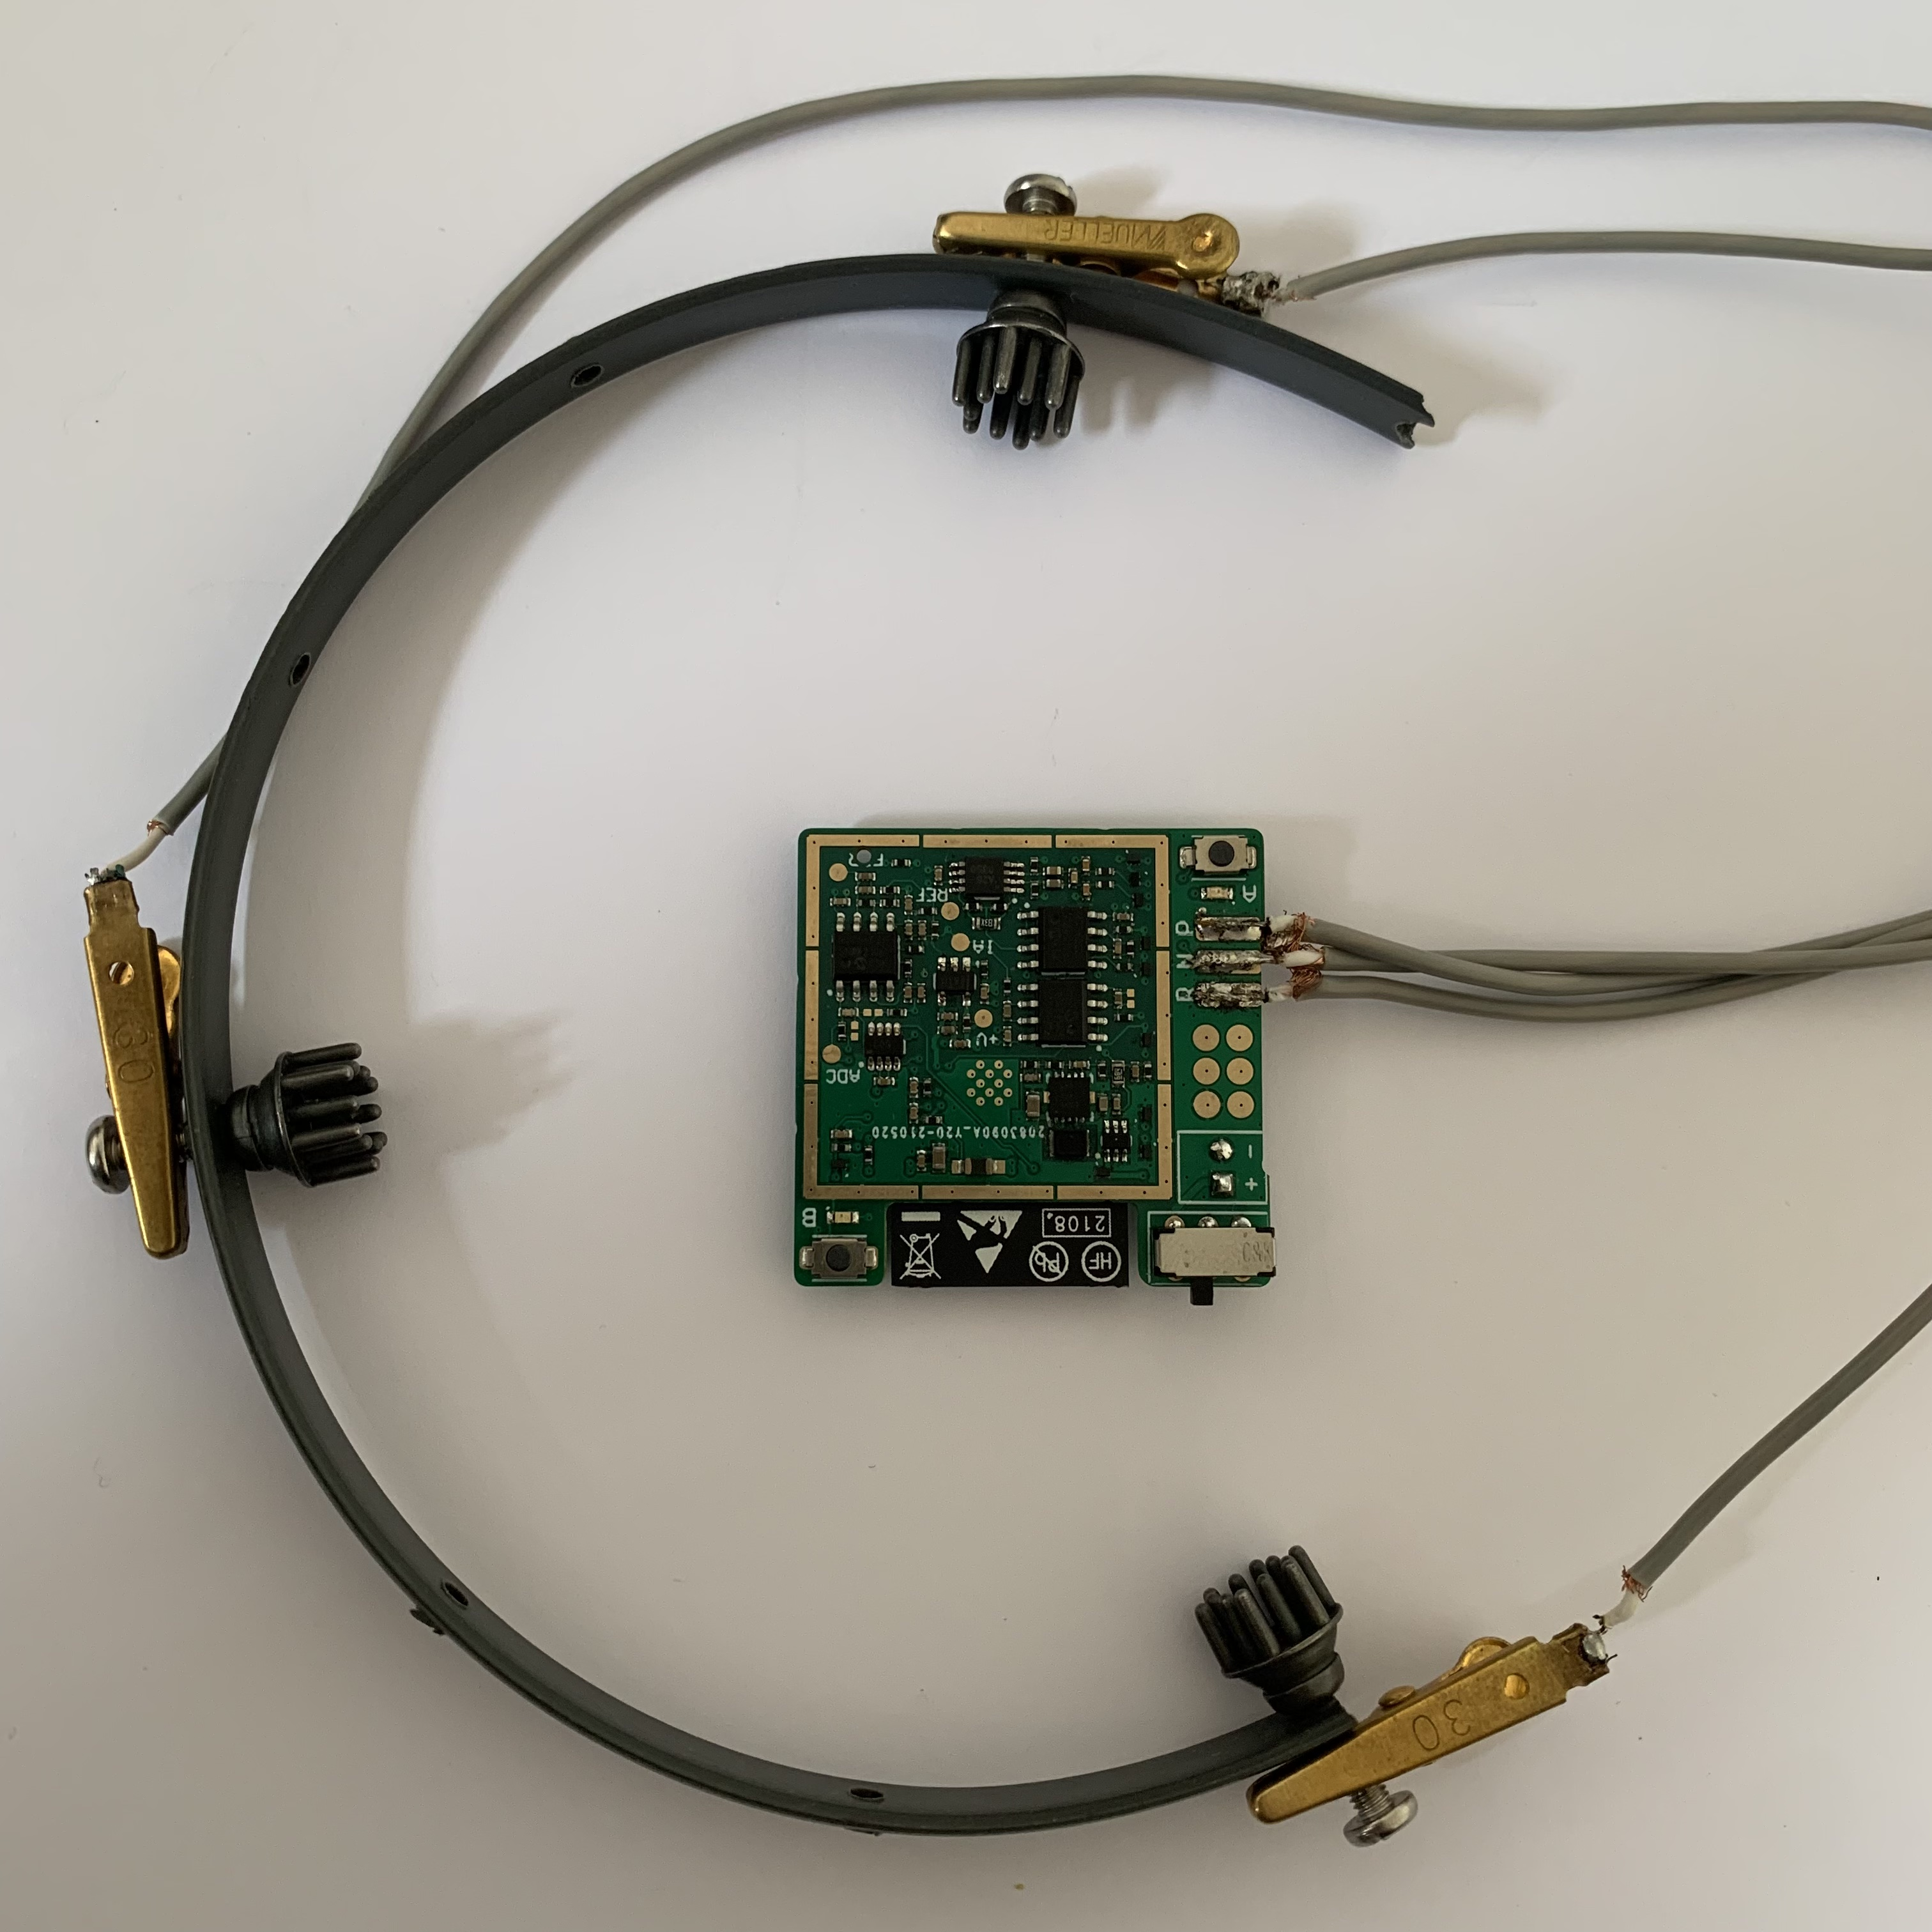
\includegraphics[width=0.6\textwidth]{frankenstein}
    \caption[A very rudimentary first prototype EEG headband]{The first very rudimentary prototype EEG band developed by the NGNI Lab based on the electronic hardware prototype in Figure \ref{fig:esp-hardware}. The active electrodes are those at the two extremes of the band and the middle one is a reference electrode.}
    \label{fig:frakenstein-hardware}
\end{figure}

\subsection{NGNI Prototype II}
Guided by the first EEG headband prototype, a second, improved version was developed by the NGNI Lab. This version, pictured in Figure \ref{fig:final-headband-subfigs}, employed a flexible and adjustable strap mechanism. This enabled the band circumference to be adjusted so as to offer greater comfort for the user and ensure appropriate contact pressure with heads of any size or morphology. Furthermore, electrodes could be adjusted more easily thanks to the 3D-printed locator structures in which they were housed. These locator structures, seen in Figure \ref{fig:final-headband-electrodes}, allowed for greatly improved contact angles between the electrodes and the scalp surface compared to the first prototype. In particular, the slight pitch and yaw flexibility introduced by the electrode locators allowed the electrodes to remain perpendicular to the undulating scalp surface, thereby maximising contact surface area. However, their stiffness also prevented excessive pitch and yaw deviations which may have arisen if the electrodes were housed directly in the flexible headband strap.

\begin{figure}
     \begin{subfigure}[c]{0.48\textwidth}
         \centering
         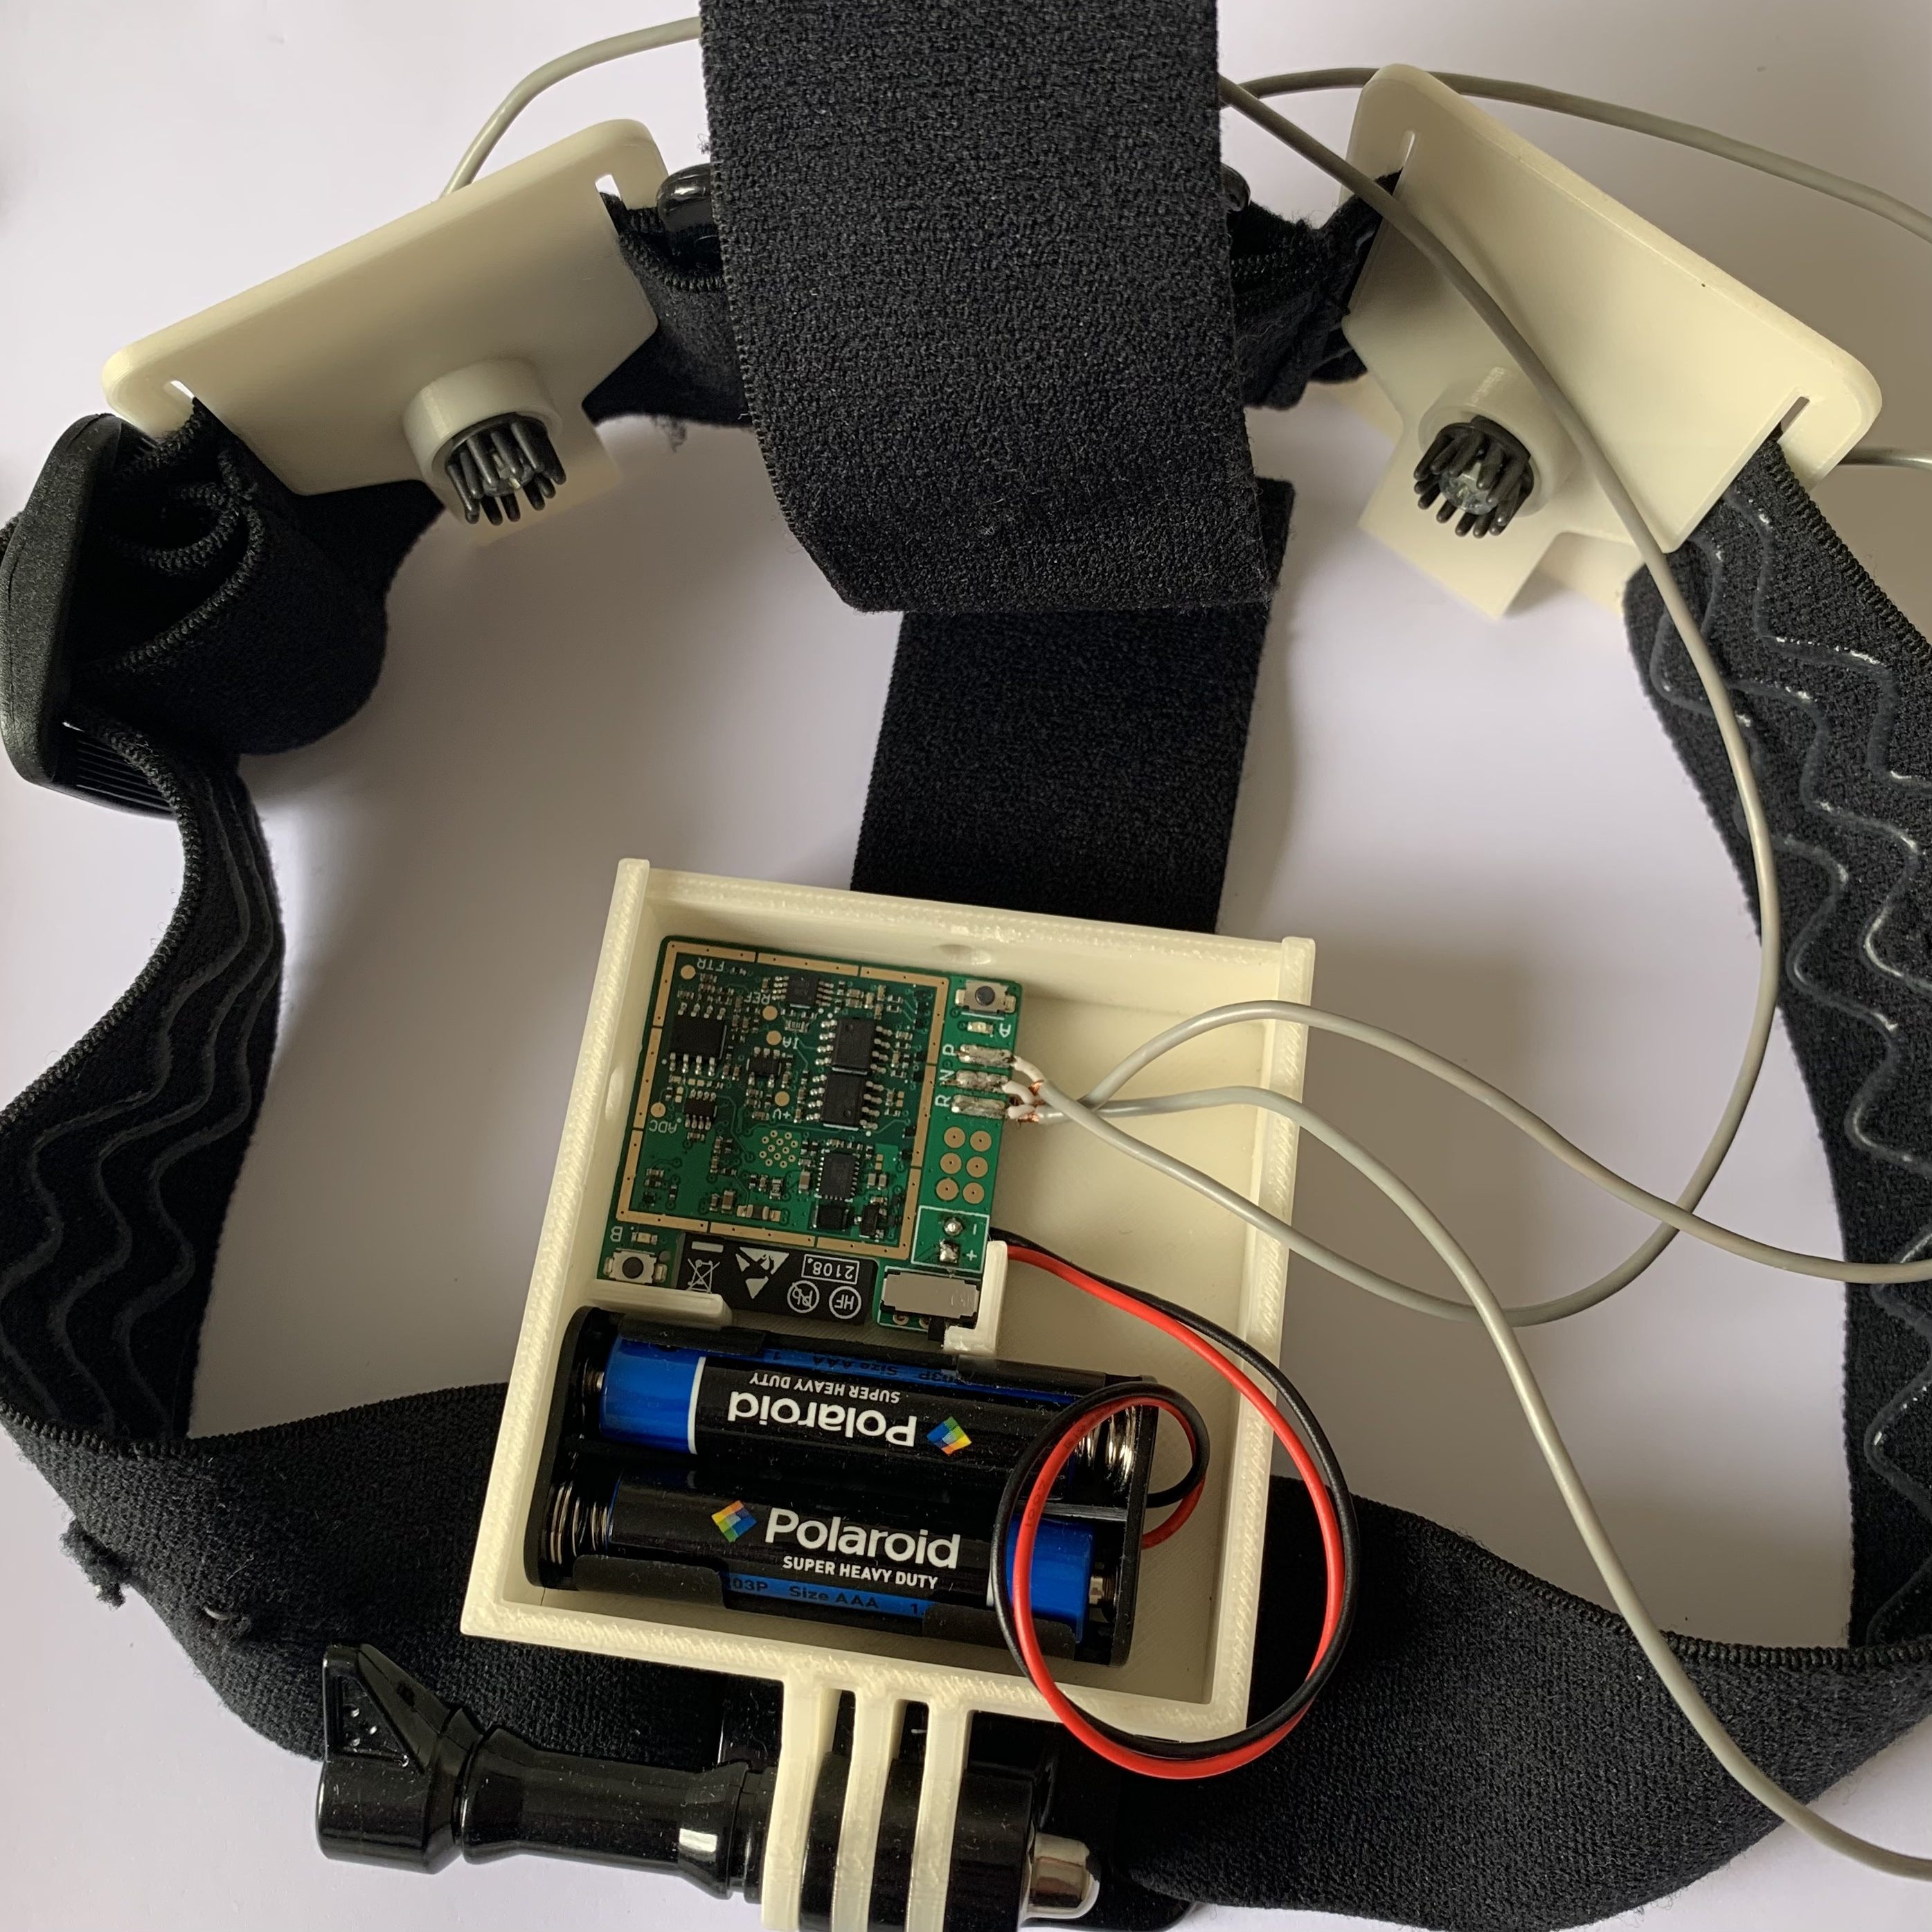
\includegraphics[width=\textwidth]{final-headband}
         \caption{View of the 3D-printed headband housing and adjustable elastic strap. The electronic hardware is externally powered by two 1.5V AAA alkaline batteries before being boosted to 3.3V using on-board circuitry.}
         \label{fig:final-headband}
     \end{subfigure}
     \hfill
    \begin{subfigure}[c]{0.48\textwidth}
         \centering
         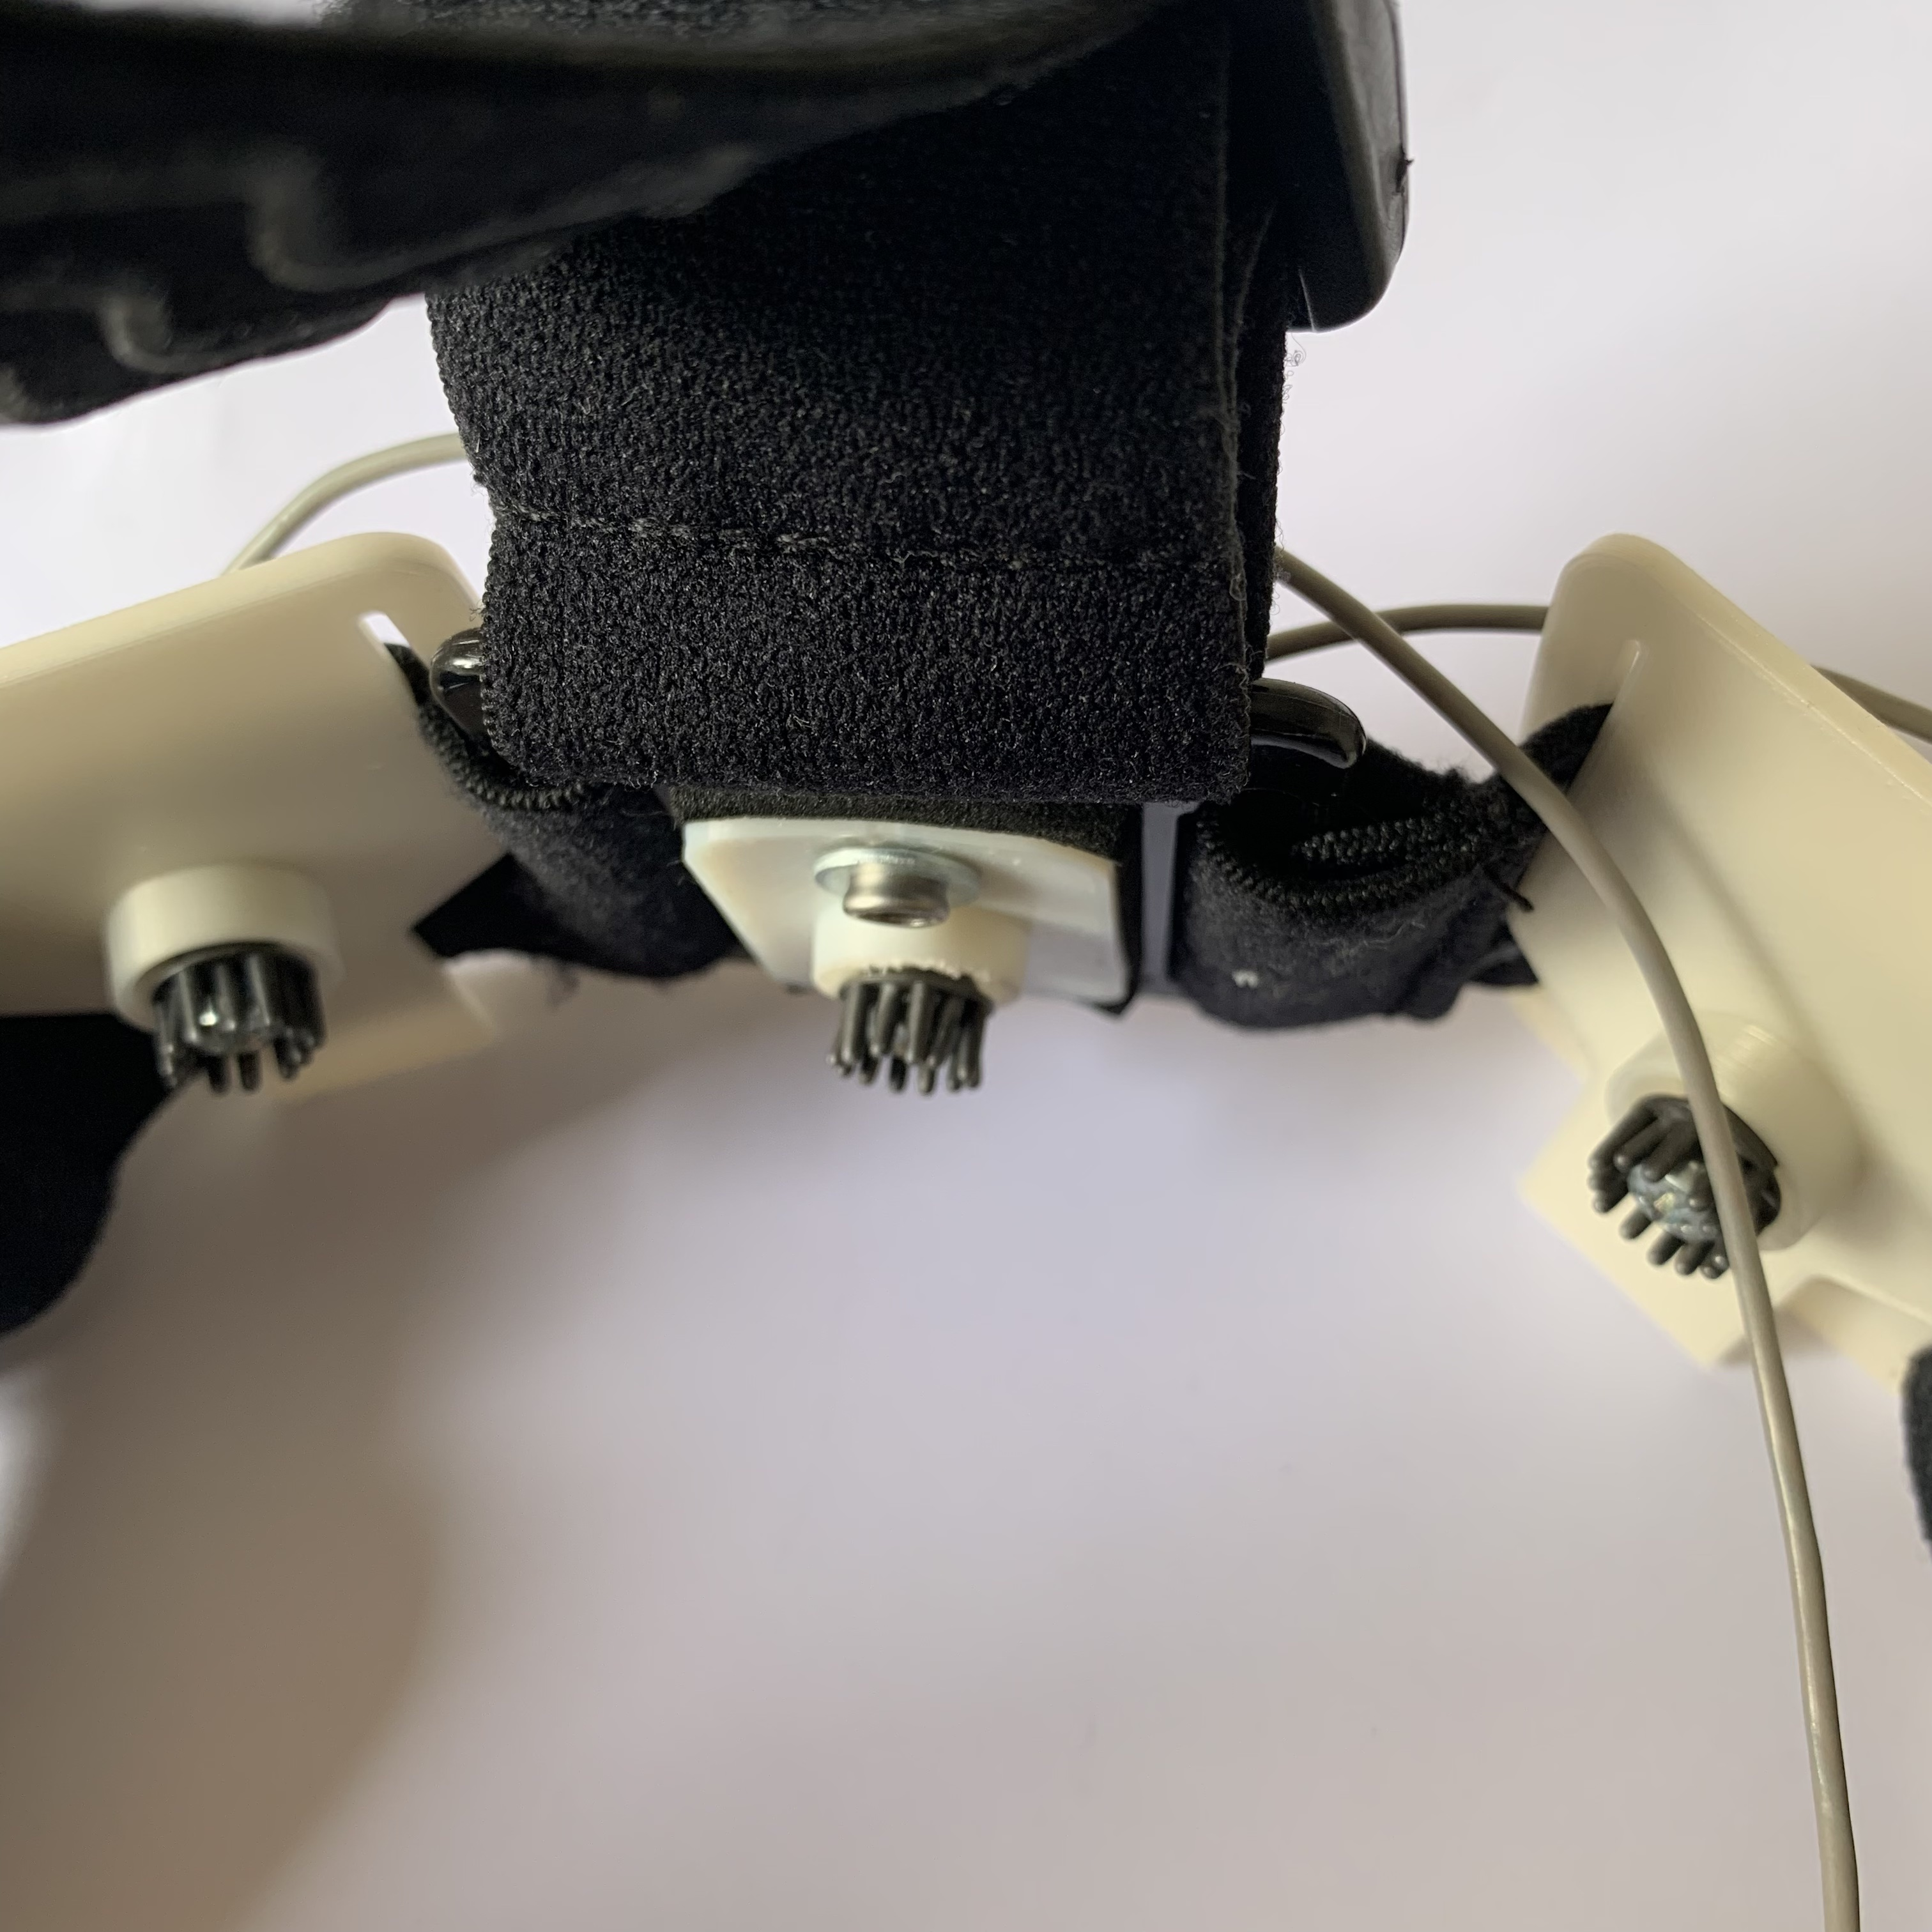
\includegraphics[width=\textwidth]{final-headband-elec}
         \caption{Close-up view of the two active electrodes on either side of the reference electrode. Electrodes are housed in 3D-printed locator structures that allow for slight pitch and yaw deviations about the axis normal to the scalp.}
         \label{fig:final-headband-electrodes}
     \end{subfigure}
        \caption{Images of the final complete hardware system comprising electronic and mechanical EEG hardware. All hardware was designed by the NGNI Lab. The band is intended to be worn such that the electrodes make contact with the back of the scalp in the occipital or parieto-occipital region.}
        \label{fig:final-headband-subfigs}
\end{figure}

\section{Experimental Procedure}
\subsection{Data acquisition}
Owing to limitations imposed by the Coronavirus Pandemic, all experimental data was recorded on the author. The SSVEP stimulus squares interface shown in Figure \ref{fig:ssvep-squares-c5} was displayed on an 11" Apple iPad Pro ($4^{\textrm{th}}$ generation, 2020) with Apple A12Z CPU, 2388x1688 px (264 PPI) display resolution and 120Hz refresh rate. The web page was displayed in the native Safari browser with no other apps running simultaneously so as to minimise CPU load and provide consistent flicker frequency across the stimulus squares. With reference to the diagram in Figure \ref{fig:visual-setup-diagram}, the iPad was positioned $d=50$cm away from the subject's visual field at an angle of $\theta=45$ degrees below the horizontal line-of-sight.

\begin{figure}[!htb]
    \centering
    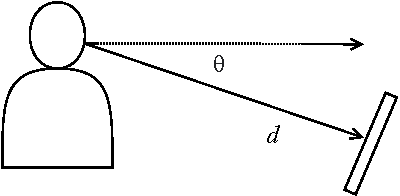
\includegraphics[width=0.3\textwidth]{visual-setup-diagram}
    \caption[Diagram showing the arrangement of the stimulus display device relative to a subject undergoing the experiment]{Diagram showing the arrangement of the stimulus display device relative to a subject undergoing the experiment. The dotted line represents the line-of-sight normal to the subject's eye line and the solid arrow is the position vector normal to the display device held distance $d$ away from the visual field at angle $\theta$ below the line-of-sight.}
    \label{fig:visual-setup-diagram}
\end{figure}

\subsection{Testing and verification}
In order to verify that signals measured from by the BCI system were valid, several checks were devised. 

\subsubsection{Basic firmware test}
The first very basic test involved verifying the integrity of the firmware on board the ESP32. This involved testing basic peripheral functionality such as toggling an LED connected to a GPIO pin and sampling a known, fixed value from the ADC. Storage and retrieval of data from flash, checking floating point precision and verifying operations from third party modules were also checked. 

\subsubsection{Alpha band test}
As mentioned briefly in Section \ref{subsection:nature-of-eeg-signals}, EEG signal energy related to visual processing typically occurs in the \textit{alpha} band between 8 and 13Hz and can be measured around the occipital region of the brain. As alpha energy is pronounced when the eyes are closed and attenuated when they are open, this phenomenon can be used as a basic test of the validity of a BCI. If signal energy as measured by the BCI in the occipital region follows this pattern, it suggests that acquired signals are not simply random noise. It should be noted, however, that individuals show varying levels of alpha reactivity and the difference in energy under these two conditions may not be significant in all individuals. 

\subsubsection{Digital signal processing tests}
In order to test the integrity of digital signal processing (DSP) elements in the BCI system (explored more in detail in Chapter \ref{chapter:system-design}), the following preliminary checks were employed. In all of the following tests, data was recorded on the electronic hardware detailed above and was analysed offline.
\begin{itemize}
    \item in order to test the on-device digital low-pass filter, data was recorded with and without the filter active. Analysis was performed to verify that signal components beyond the target frequency band were suitably attenuated and that pass-band distortion was acceptable. 
    \item in order to verify the equivalence between original and down-sampled versions of the same signal, data was collected under three conditions: (i) sampling at $f_s=256$Hz with low pass filtering but no downsampling, (ii) sampling at $f_s=256$Hz with low pass filtering and downsampling to $f_s'=64$Hz and (iii) sampling at $f_s=256$Hz with \textit{no} low-pass filtering and downsampling to $f_s'=64$Hz.
\end{itemize}

\subsubsection{Artificial signal decoding test}
In order to test the hardware and signal decoding elements, a square wave signal at a known frequency $f_0$ was produced and applied across the active electrodes. The resulting signal spectrum was measured and compared to the theoretical spectrum of a square wave at frequency $f_0$. This was performed with and without low-pass filtering to determine if high frequency harmonics were being attenuated correctly. SSVEP signal decoding algorithms were also tested by ensuring that they produced a decoded output matching the artificial stimulus frequency $f_0$.

\subsection{Demonstration procedure}
During the Royal Society exhibition, audience members attending remotely from various locations will be presented a mobile-friendly, lightweight web page with two or three flickering squares that will form the SSVEP stimuli. These squares will be programmed to flicker at predetermined stimulus frequencies $f_1, \dots, f_n$. Each stimulus will correspond to an action - such as `up' or `down' - that will control an avatar in a cooperative multiplayer game or simulation. The core objective of the designed BCI system is to decode $f_1, \dots, f_n$ in order to interpret each user's desired action (i.e. discern which stimulus square they are focused on).